% For any doubt:
% https://www.overleaf.com/learn/latex/How_to_Write_a_Thesis_in_LaTeX_(Part_1):_Basic_Structure

\documentclass[12pt,twoside]{book}
% This book is the official final thesis document

% Required package definition
\usepackage[utf8]{inputenc}
\usepackage{graphicx}
\usepackage[a4paper,width=150mm,top=25mm,bottom=25mm, bindingoffset=6mm]{geometry}
\usepackage{fancyhdr}
\pagestyle{fancy}

\setcounter{tocdepth}{4}
\setcounter{secnumdepth}{4}

% Image path definition
\graphicspath{ {images/} }

% This is how our cover is gonna look like
\title{
{Thesis Title}\\
{\large Politecnico di Milano}\\
{
\includegraphics[width=3cm, height=4cm]{university.png}}
}
\author{Carlos Blasco Andrés}
\date{\today}


\begin{document}

\maketitle

\chapter*{Abstract}
Abstract goes here

\chapter*{Dedication}
To mum and dad

\chapter*{Declaration}
I declare that..

\chapter*{Acknowledgements}
I want to thank...

\tableofcontents
\listoftables
\listoffigures

\chapter{Introduction}
This is a test.
\section{Section 1}
This a test for the first section.
\section{Section 2}
And this is a test for the second section.


\chapter{State of the Art}
% Make an introduction to the chapter describing what I am gonna speak about.

\section{Data-Intensive Applications}

Data-Intensive Applications (DIAs) are a class of parallel computing applications which handle high amount of datasets and that devote the most of their processing time to I/O and manipulate such datasets. These kind of applications are able to manage datasets of several terabytes and petabytes which are available in a wide variety of formats and that are distributed among several locations. This capability to process large volumes of data is possible due to the fact that DIAs use multi-step analytical pipelines with transformations and fusion stages in order to parallelize the execution of the data.

Intensive applications can be classified according to the parallel processing approaches commonly known as compute-intensive and data-intensive. On the one hand, compute-intensive is used to describe application programs that are compute bound. Such applications devote most of their execution time to computational requirements and they process small volumes of data. In this kind of applications, processes must be parallelized by means of individual algorithms and then they must be decomposed into separate tasks. Later, such tasks are executed in a pipeline reaching higher performance that in serial processing. Finally, compute-intensive applications are able to perform multiple operations simultaneously as they allow task parallelism.

On the other hand, data-intensive is used to describe application programs that are I/O bound. Such applications devote most of their execution time to I/O, move and manipulate the datasets. This second parallel processing approach, unlike compute-intensive, processes large volumes of data. Data-intensive applications require the partition or subdivision of the initial dataset in some smaller datasets due to the fact that the large volume of data that they are composed. These partitions must be processed independently by the application allowing the parallelization of the initial dataset. Once the partitions are executed, they must be reassembled in an output dataset.

As any type of application which takes advantage of data-parallelism, DIAs need to select an algorithm not only to distribute data among the processing nodes of the cluster but also to execute the data in such processing nodes. Moreover, they need to adopt a strategy to decompose the datasets, find a trade-off in terms of working loads in the processing nodes by means of load balancing systems and to communicate the nodes of the cluster.

\subsection{Characteristics}

Data-intensive applications are modeled in a different way than any other computing application due to the property of DIAs to be processed in a cluster infrastructure. Moreover, as any other system, DIAs need to reach a high performance in order to be make our application efficient; this is possible by means of the minimization of the number of movements of the data. Other important properties required by DIAs are that they must be available when they are called, annd that they must be reliable to the number of failures; both properties are accomplished due to data-intensive applications are fault resilient. Last but not least, data-intensive applications must be able to change the number of required nodes taking into account the workload. Then, four characteristics can be defined in order to distinguish data-intensive applications from any other kind of computing system:

\subsubsection*{Dataflow Model}

Data-intensive applications are modeled by means of nodes where some transformations take place and data or programs flow between such nodes. Moreover, such model allows to control how to schedule, to execute, to balance the load and to communicate programs and data during runtime using a cluster computing infrastructure.

\subsubsection*{Data Movement Minimization}

Minimize the number of movements required by each data along the different computations in order to achieve high performance is crucial in data-intensive applications. Then, processing algorithms are executed on the nodes of the dataflow model where the data is located, reducing the number of movements and therefore increasing performance.

\subsubsection*{Fault Resilient}

Due to the fact that DIAs work with high amounts of data, the probability for the hardware to fail is greater than in other computing systems but the same happens with the probability of communications errors and software bugs. This is why, DIAs are designed to be fault resilient. In order to make these applications available and reliable, on the disk of the storage of such systems redundant copies of all data files or intermediate processing results can be found. But also they are provided with systems capable to detect the failure of any node or processing failures and, once such failures are detected, then re-compute the results.

\subsubsection*{Node Variability}

Depending on the hardware and software architecture of the data-intensive application, the required number of nodes and processing tasks and its variability along the runtime can be fix or variable. This is due to the fact that it is very important to achieve a comfortable processing independently of the amount of data and, also, to reduce the critical time of computation by adding some nodes.

\subsection{Frameworks}
\subsubsection{Apache Hadoop}

Apache Hadoop is an open source software framework that supports distributed applications. As any other DIA, Hadoop allows to work with thousands of nodes and petabytes of data. This framework is composed by a processing layer called MapReduce which was inspired by Google documentation.

MapReduce works as a DIA processing large volumes of data. First of all, this programming model divides the incoming works into a set of independent tasks and, after that, such tasks are executed. Then, the user sends the complete job to a master which divides it into independent tasks and submits them to the slaves in order to process the works in parallel. This process allows Hadoop to reach speed and reliability of cluster.

In summary, Hadoop MapReduce works breaking the incoming datasets into independent sets that are executed in parallel by means of two phases: map phase and reduce phase. Firstly, in the map phase, we specify the business logic putting the custom code in the way MapReduce works. And, secondly, in the reduce phase, we specify processing like summations and aggregations.

\subsubsection{Spark}

Spark is an open source platform that allows general-purpose and fast cluster computing. It is an engine that allows to process large volumes of data.

Spark enables users to access repeatedly to datasets in order to perform streaming, machine learning or SQL workloads by means of high-level APIs in Java, Scala, Python and R. It also allows users to accomplish batch processing or stream processing.

Moreover, Spark can be integrated with any other data-intensive tool due to its design. Spark is compatible with Hadoop as it is able to access Hadoop data sources and run on Hadoop clusters. This platform extends MapReduce, the engine of Hadoop, by including iterative queries and stream processing.

Some features make Spark more efficient than Hadoop. The following features make Spark being the 3G of Big Data:

\begin{itemize}

\item Fault tolerance.
\item Dynamic in nature.
\item Reusability.
\item Advanced analytics.
\item Lazy evaluation.
\item Real-time stream processing.
\item In-memory computing.

\end{itemize}

The in memory computing feature reduces the number of read-write to disk operations what achieves a data processing performance 100 times faster in memory and 10 times faster on the disk. Due to the high amount of operators that Spark provides, to achieve parallel applications is easier with Spark. Regarding to fault tolerance, Sparks handles the failure of the nodes in the cluster by means of Resilient Distributed Datasets (RDDs) which its specific design makes to reduce the number of failures to zero.

In conclusion, Spark can be differentiated from Hadoop in its cluster management system. On the other hand, regarding to the similarities between Spark and Hadoop, Spark takes advantage of Hadoop for storage.

\subsubsection{Apache Flink}

Apache Flink is an open source platform which allows data streaming computation because of its data flow engine. Moreover, as happens with Spark, Apache Flink is able to execute stream processing and batch processing and it is also compatible with Hadoop.

Apache Flink can undertake efficiently some different types of processing, becoming in the most potent open source platform in the market to handle them. Such processing types are:

\begin{itemize}

\item Batch Processing.
\item Interactive processing.
\item Real-time stream processing.
\item Graph Processing.
\item Iterative Processing.
\item In-memory processing.

\end{itemize}

Apache Flink reduces the complexity that other platforms as Spark faced by means of some improvements. Among such improvements highlight the integration with MapReduce of query optimization, some concepts from database systems and efficient parallel in-memory and out-of-core algorithms. These optimizations are given due to the fact that Flink architecture is designed taking into account the streaming model. Such design improves the micro-batch approach taken in Spark for data streaming processing making Flink faster and with lower latency for such kind of processing.

Following the example of Spark, Apache Flink is provided with three APIs (DataStream, DataSet and Table APIs) in order to use its engine. DataStream and DataSet APIs are two regular programs used by Flink in order to perform transformations on data streams (filtering, aggregating, update state...) and data sets (joining, grouping, mapping...) respectively. On the other hand Table API is used for relational operations and it can be integrated into DataStream API for relational stream processing and into DataSet API for relational batch processing.

Finally, it is important to remark the five features that Apacha Flink presents:

\begin{enumerate}

\item Low latency and high performance.
\item Fault tolerance.
\item Memory management.
\item Iterations.
\item Integration.

\end{enumerate}

All these characteristics are what make Flink the 4G of big data and the most powerful tool when dealing with data stream processing.

\section{Privacy Policies in IT}

Computer security, also known as cybersecurity or information technology security (IT security), is the protection of computer systems and networks from people who is interesting in stealing or damaging their hardware, software or the data with which they are working.

Every computer security system accomplish the well-known CIA paradigm. "C" stands for Confidentiality, "I" for Integrity and "A" for Availability and they are the three basic requirements that compose such paradigm. Any computer security system has to grant that any piece of data has to be accessed only by those who are authorized, accomplishing such requirement, information is confidential. Moreover, such systems have to be able to allow data modifications only to those how are authorized for it and only in the way that they are entitled to modify them, this requirement makes information to be integrated. Finally, data must be available to everyone who has a right over them within some time constraints, this makes information to be available. These three requirements raise an engineering problem and it is that availability conflicts with confidentiality and integrity due to the fact that if a data is available then it could not be confidential as anybody may modify it and it could not be integrated as anybody could modify then. This is the main problem that has to be faced when designing computer security problems. In order to handle this complex engineering problem, designers can use legal instruments but also technical tools.

Due to the fact that the information of many entities (persons, companies, etc.) are involve in such complex problem, there are some legal instruments to handle the design of security systems. This is the case of privacy policies. Privacy policies are statements or legal documents that reveal how an entity can collect, use or handle data from another entity. Privacy policies can differ from one country to another this is why there are some agreements in order to handle them. In the European Union (EU) the General Data Protection Regulation (GDPR) is in charge of harmonizing data privacy laws across all member states of the EU. In spite of these regulations, there are many ways in order to apply privacy policies.

On the other hand, when a computer security system is designed, the designer has to put himself in the place of the cyberthief, or threat agent, in order to achieve a secure system. Such cyberthiefs try to find vulnerabilities and, then, exploit them in order to steal some information. Usually, vulnerabilities are a bug that allows to violate the CIA paradigm but the exploit can be a wide variety of vulnerability uses. Despite this design technique, unfortunately, a great amount of vulnerabilities are found when users accidentally deal with the applications once the applications are in the market.

Another remarkable point is the importance of threats, that are potential violations of the CIA paradigm, in computer security systems. This means that an information system can be seen its security system broken due to the fact that a circumstance or an event could impact on it adversely by means of the break of any of the three basic requirements of a computer security system. A threat is composed by three layers. The attacker or threat agent that is the person or the information system that performs the attack action, the countermeasure layer that is all the systems that try to identify an attack and stop it and, finally, the target of the attack that is on which resides the vulnerability and on the threat consequences take place when the exploit arrives to the vulnerability.

In conclusion, the concept of computer security involves many fields but when dealing with the design of DIAs, it is very important to take into account not only the CIA paradigm but also the design techniques from the threat agent perspective in order to reach secure DIAs, always under the legal framework of privacy policies. Furthermore, what makes security on DIAs reliable is the balance on its conflicting requirements what is a complex engineering problem. Finally, systems with a high amount of vulnerabilities but with no threats, are secure systems. However, systems with many threats and only a few vulnerabilities become in the most attacked systems and, then, the ones that need more security measures.

\subsection{Privacy Policies in DIAs}

Due to the fact that DIAs are constantly managing data from different entities, it is very important the way in which privacy policies are applied on them. The final goal of applying them is that, in case of threats, threat agents cannot obtain such data. This reduces the probability of threats as there is no sensitive data that can be obtained and, then, the CIA paradigm cannot be broken.

When dealing with DIAs, sensitive data are sent in data streams. Such data streams are composed of tuples which can contain a high variety of data. Each tuple of a data stream contains a finite set of data that are always ordered in the same way. Due to the fact that all the tuples contained in a data stream have the same structure, when speaking about data streams, each of the data of the tuple is considered as a field of the data stream. Due to this distinction on the fields of the data streams, data streams can be classified into three different sets:

\begin{itemize}

\item Subject-specific streams.
\item Subject-generic streams.
\item Non-personal streams.

\end{itemize}

A subject-specific stream is a stream composed of a field referring to the data subject. This means that each tuple of the stream contains a data which is the owner of the tuple. A subject-generic stream is a stream without data subject. However, subject-generic streams are produced by an operator whose input is a subject-specific stream. Finally, a non-personal stream is a stream without data subject and that it has not been produced by an operator whose input is a subject-specific stream.

The context in which a tuple is conveyed is also important. Depending of the context in which data are transferred, an entity could want that the data of the tuple are private or public. This context is specified by means of three variables:

\begin{itemize}

\item Observer.
\item Role.
\item Purpose.

\end{itemize}

The first variable is the observer of the data, the entity who demands the usability of the data. The second variable is the role that the requesting entity is playing. The requesting entity can be a person but also a company. In the case of the company, many persons working for such company can be demanding the data of the tuple and each person has a role inside the company, this is why the role is an important variable in order to define the context in which a privacy policy can be applied. Finally, the third variable that defines the context is the purpose. The purpose for which the requesting entity demands the data of the tuple. Then, the context in which a privacy policy has to be applied is defined by means of three variables that are called static context variables (SCV) as, once they are defined, they are not going to change and because of this they are static.

Another important distinction is the one given by the data that compose a tuple. Each of these data can be strings or numbers. Because of this, a classification on the type of each data of the tuple, and then on the type of the fields of the streams, has to be defined. Moreover, following the approach given by the SCVs, each of these values are considered as a variable as the values of a field of a given stream can change depending on the tuple that is referred. Then, the variables that compose a field of a stream are:

\begin{itemize}

\item Categorical variables.
\item Numerical variables.

\end{itemize}

Categorical variables are those that correspond to a string in any programming language. They can be words but also links or any set of letters with special characters and numbers. The second type of variables correspond to numbers but also to a range which corresponds to a pair of numbers. For example, a data subject can be a categorical variable when it is the name of the user who uses the DIA but a data subject can be also a numerical variable if it is an ID which is compose only by numbers. Furthermore, the set of categorical and numerical variables used by a DIA are called contextual variables.

Taking into account these three classifications, privacy policies can be defined by means of some rules. These rules have to be defined making a relationship between the contextual variable used by the DIA and some values that the user selects in order to encrypt the original fields of the stream. These relationships are made by means of logical operators. In the case of categorical variables, the operators that can be used are: equal to ($=$) and not equal to ($\neq$). On the other hand, in the case of numerical variables, the relation operators that can be used are: equal to ($=$), not equal to ($\neq$), is greater than ($>$), is less than ($<$), is greater than or equal to ($\geq$) and is less than or equal to ($\leq$)

Finally, due to the fact that privacy policies encourage the anonymity of the entity who owns the data of the tuple, depending on the data stream classification explained above and the rules defined by each user, privacy policies can differ. Then, another classification can be made, in this case about the privacy policies in DIAs:

\begin{itemize}

\item View Creation Policies (VCPs).
\item Data Subject Eviction Policies (DSEPs).

\end{itemize}

\subsubsection{View Creation Policies (VCPs)}

View Creation Policies (VCPs) are a type of privacy policies for DIAs which are applied to subject-specific streams. VCPs are applied when the context is precisely specified by means of the SCVs and the information contained in all the fields of the stream is observable, which means that it has not been modified before by another privacy policy.

Furthermore, VCPs are defined by means of a set of rules which are relationships between the contextual variables used by the DIA and some values that the user selects in order to encrypt the original fields of the stream. In this kind of privacy policies, the encrypted final values of the stream are defined by means of generalization vectors. A generalization vector defines the value to be used in order to generalize each of the fields that compose a subject-specific stream.

In conclusion, given a tuple belonging to a subject-specific stream, if at any instant such tuple satisfies all the rules defined by means of logical operators relating some contextual variables with a value defined by the user of the DIA, a generalization vector is applied on the tuple in order to generalize each of the fields of the streams and obtaining an encrypted tuple. Then, a VCP is defined by means of four items:

\begin{enumerate}

\item Subject-specific stream.
\item Data subject.
\item Set of relational rules.
\item Generalization vector.

\end{enumerate}

\subsubsection{Data Subject Eviction Policies (DSEPs)}

Data Subject Eviction Policies (DSEPs) are applied when given an operator, which input is a subject-specific stream, produces a subject-generic stream. Sometimes, the entity who owns the data which are flowing along the DIA does not want that an operator takes some information from the input stream in spite of the output stream is not showing any information directly pointing to such owner. This is the case in which DSEPs are applied.

Unlike what happens with VCPs, DSEPs do not encrypt the fields of a given data stream. In this case, DSEPs prevent the tuples flowing in the subject-specific stream that inputs into a given operator from being processed by such operator. In this case, the output from the operator is computed without taking into account the data of the data subject who defines the DSEP, preserving the anonymity of the owner of the data for the computation of a certain statistic.

In conclusion, in order to define a DSEP, first of all, a set of rules have to be specified by the user relating some contextual variables with some values that such user has to define. Then, given an instant when all the defined rules are satisfied on a subject-generic stream which outputs from a given operator, all the tuples referring to the data subject who defined such rules have to be evicted from the subject-specific stream that inputs into the given operator. Then, a DSEP is defined by means of three items:

\begin{enumerate}

\item Subject-generic stream.
\item Data subject.
\item Set of relational rules.

\end{enumerate}

\section{Modeling \& Metamodeling}

A model is a representation of a reality in order to explore, to redesign or to transform it. This representation can be externalized by means of a diagram in a paper or in a computer software. Modeling is the method that has to be developed in order to reach a model. A modeling method consists of a modeling technique and a mechanism or algorithm working on the model. Moreover, a modeling techniques consists of a modeling language and a modeling procedure. A modeling procedure is a sequential process composed of several steps but also an iterative process since the procedure can be repeated many times until the final model is reached. In spite of several modeling procedures can be accomplish in order to create a model, all these approaches share some common steps:

\begin{itemize}

\item Purpose definition.
\item Boundaries definition.
\item Model elements definition.
\item Relationships definition.

\end{itemize}

The first step that has to be accomplished in order to create a model is to define its purpose. With such purpose, the questions that the model will have to answer, once it is implemented, should be specified. Later, the boundaries of the model must be specified. Such boundaries must focus on the reality that has to be modeled discarding any information that is not able to reach the predefined purpose. Once these boundaries are defined, everything that is going to take part of the model is called the model domain. Due to the fact that usually this domain is still very big, each concept belonging to the model domain must be filtered taking into account the relevance of each of them and grouping those concepts that are identical in order to reach the purpose. After that, each of the groups with identical concepts can be transformed into a model element, which is an abstraction of all the concepts that are part of the group. Finally, the relevant relationships among the model elements have to be identified and represented in the model.

Furthermore, a model must be complete in order to be able to answer the question specified in the purpose but also, it must be consistent which entails the lack of contradictions in its representation. In order to reach such characteristics, modeling methods take advantage of modeling techniques in addition to a mechanism, an algorithm, working on the model.

The first component of a modeling technique that is a modeling language is a set of well-known elements and relationships by means of which a model can be represented. A modeling languages is described by a syntax, semantics and a formal notation. A syntax is the set of elements, relationships and rules that can be written in order to represent a model by means of a grammar. Moreover, a syntax can be described by two different types of grammars: graph grammars and metamodels. A metamodel is a model of a modeling language. A metamodel is written by means of a modeling language that is known as the metamodeling language. The metamodeling language has a model which defines it. This is why exists a modeling hierarchy which is not limited and that ends given a useful abstraction level of the model. In the table \ref{Modeling Hierarchy} there is an example of a modeling hierarchy with five levels.

\begin{table}[h!]
\centering
	\begin{tabular}{||c|c|c||} 
	\hline\hline
	Language Level & Models & Language Name \\ [1ex] 
	\hline\hline
	Level 1 & Model & Modeling Language  \\
	\hline
	Level 2 & Metamodel & Metamodeling Language  \\
	\hline
	Level 3 & $Meta^2$-Model & $Meta^2$-Modeling Language  \\
	\hline
	Level 4 & $Meta^3$-Model & $Meta^3$-Modeling Language  \\
	\hline
	Level 5 & $Meta^4$-Model & $Meta^4$-Modeling Language  \\
	\hline\hline
	\end{tabular}
\caption{Modeling Hierarchy}
\label{Modeling Hierarchy}
\end{table}

The semantics of a modeling language describe the meaning of the language by means of a semantic domain and a semantic mapping.

Finally, the formal notation describes how the modeling language is visualized. Some symbols are used in order to represent the represent the syntax of the language in a diagram.

On the other hand, the finality of the mechanism is to check that the model written with the modeling language by means of the modeling method is correct and satisfies the purpose of the model. There are three main types of mechanisms and algorithms: generic, specific and hybrid.

In the figure \ref{fig:Modeling Method Components} o model of a modeling method is shown.

\begin{figure}
\centering
{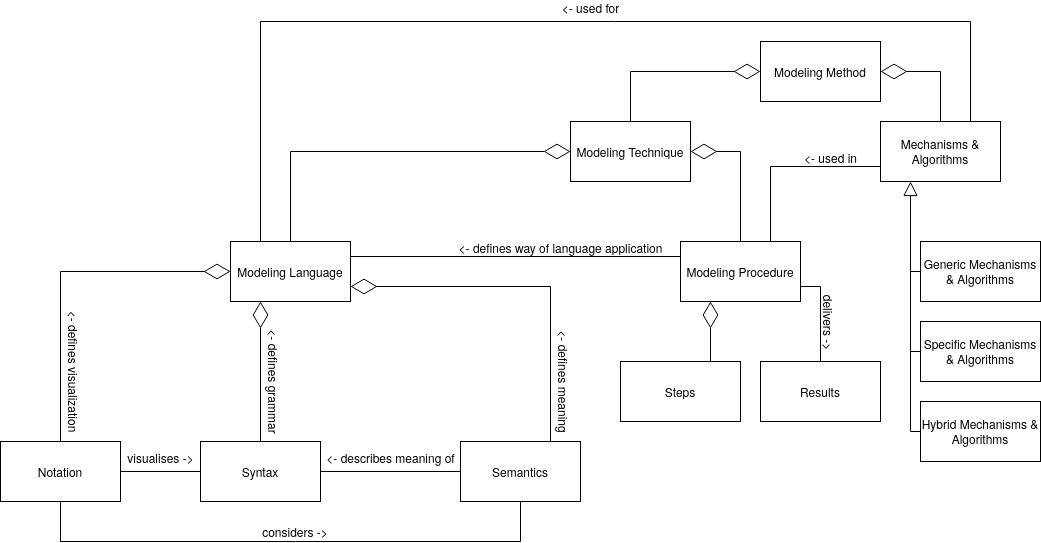
\includegraphics[scale=0.3]{./chapter2/compModelMethod.png}}
\caption{Modeling Method Components}
\label{fig:Modeling Method Components}
\end{figure}

\subsection{Unified Modeling Language (UML)}

Unified Modeling Language is a standardized modeling language whose objective is to provide system architects, software engineers, and software developers with tools for analysis, design, and implementation of software-based systems as well as for modeling business and similar processes.

UML is able to achieve such goal by means of a wide variety of options to build modeling diagrams. Among the fourteen possibilities that UML provides to construct a diagram, a distinction between two main classes can be made: behavior diagrams and structural diagrams.

Behavior diagrams represent the dynamics of a system, this means the representation of all the possible changes that a system can experience over time. This class is composed of seven diagrams: activity diagram, communication diagram, interaction overview diagram, sequence diagram, state machine diagram, timing diagram and use case diagram.

On the other hand, structural diagrams represent the different static parts of the system, that ones which do not change over time. This representation can be done from different abstraction and implementation levels and making the corresponding relationships between the parts of the system. This second class is composed of other seven possibilities for diagram construction: class diagram, component diagram, component structure diagram, deployment diagram, object diagram, package diagram and profile diagram.

A UML diagram making a description of all the UML diagrams can be seen in the figure \ref{fig:UML Metamodel}.

\begin{figure}
\centering
{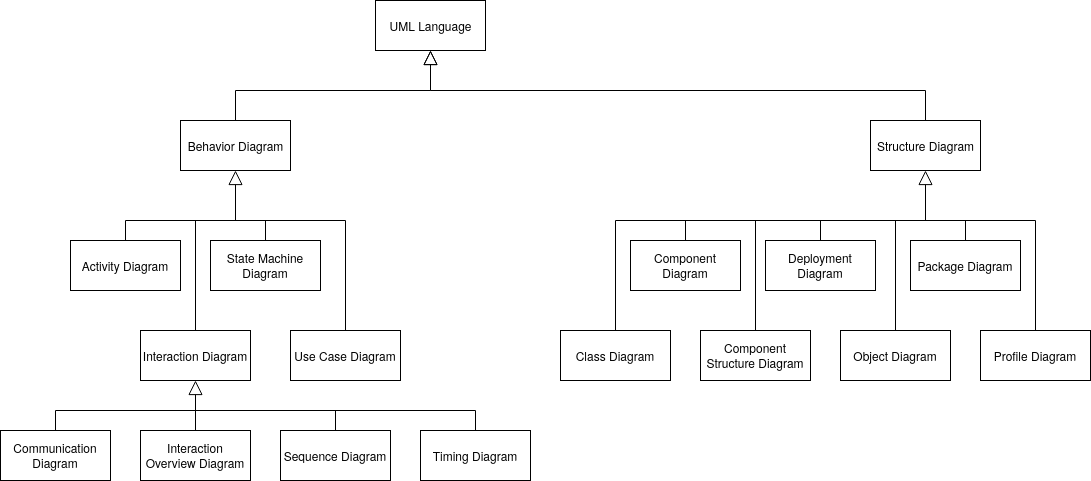
\includegraphics[scale=0.3]{./chapter2/umlMetamodel.png}}
\caption{UML Metamodel}
\label{fig:UML Metamodel}
\end{figure}

\subsubsection{Class Diagram}

This kind of diagram represents the model elements and the relationships that exist between such elements. The model elements, which are represented by means of nodes, can be: class, component, data type, interface, model or package among others. Regarding to the relationships between the nodes, they can be: association, association class, dependency, generalization or information flow among others.

Class diagrams are commonly used to represent the metamodel of the syntax of a modeling languages. Due to the fact that this kind of diagrams is not able to fully express syntactical rules, usually they take advantage of constraint languages as Object Constraint Language (OCL).

























\chapter{Requirements and Design}
The first requirement that is needed in order to develop the big data application is to install the corresponding versions of Eclipse, Papyrus and Acceleo. In spite of the application is able to work with other versions, some problems could appear because of the changes that they present. The models implemented in this document have been develop with the following versions:

\begin{itemize}

\item Eclipse 2019-03 (4.11.0).
\item Papyrus SysML 1.4 Feature	1.3.0.
\item Acceleo 3.7.8.201902261618.
\item m2e-Maven Integration for Eclipse (includes Incubating components) 1.11.0.20190220-2119.
\item Apache Flink 1.4.0.

\end{itemize}


\chapter{Solution}
In order to implement the application, first of all, a new project has to be created in Eclipse. This project is going to be a Papyrus project (figure \ref{fig:Papyrus Project}).

\begin{figure}
\centering
{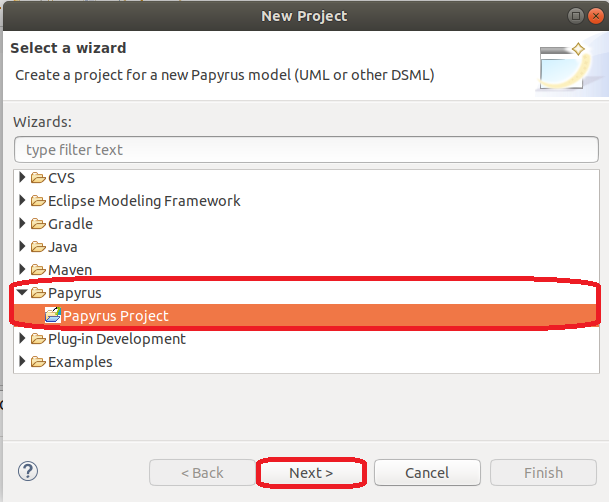
\includegraphics[scale=0.3]{./chapter4/projPapyrus/Selection_001.png}}
\caption{New Papyrus Project}
\label{fig:Papyrus Project}
\end{figure}

The first field that has to be specified is the Architecture Context. Here, the default values are the right ones as an UML model is what is required to implement with Papyrus (figure \ref{fig:Architecture Context}).

\begin{figure}
\centering
{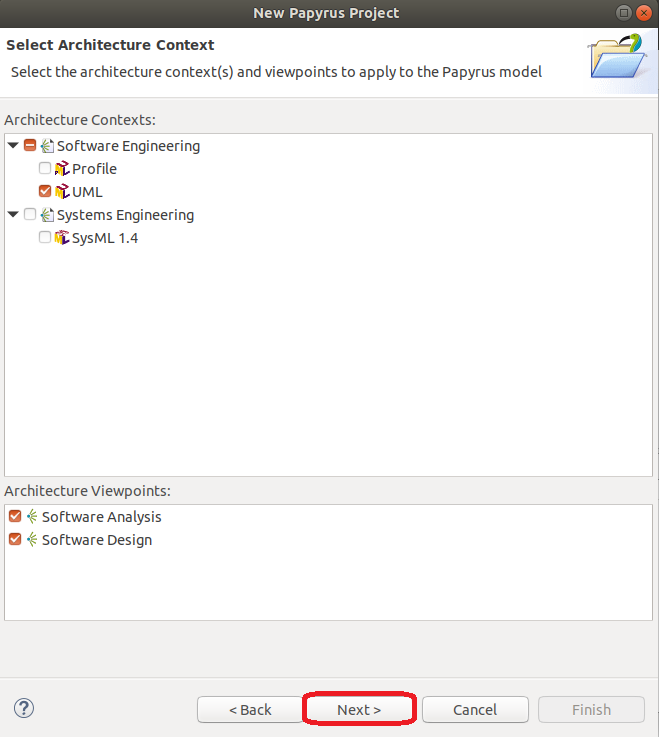
\includegraphics[scale=0.3]{./chapter4/projPapyrus/Selection_002.png}}
\caption{Architecture Context}
\label{fig:Architecture Context}
\end{figure}

After that, the name of the project has to be defined. Due to the fact that it is going to implement an application called Great Seller, the name of the Papyrus project is going to be greatSellerApp (figure \ref{fig:Project Name Definition}).

\begin{figure}
\centering
{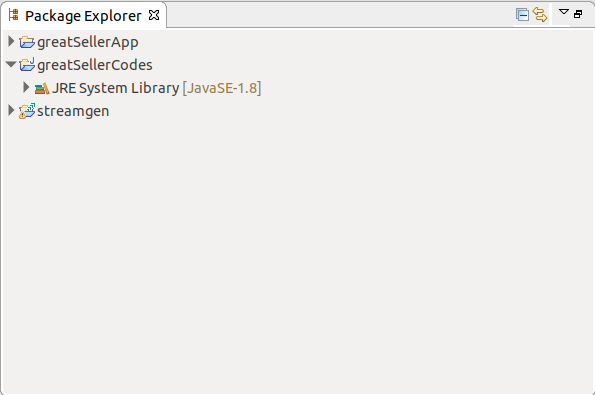
\includegraphics[scale=0.3]{./chapter4/projPapyrus/Selection_003.png}}
\caption{Project Name Definition}
\label{fig:Project Name Definition}
\end{figure}

The next step is to select the representation kind and to choose the StreamGen profile. StreamGen requires Papyrus to make a class diagram representation and, as the StreamGen project is already in the Eclipse workspace, the profile can be found browsing in the workspace (streamgen/profile/StreamUML.profile.uml). As it can be seen in the figure \ref{fig:Representation Kind}.

\begin{figure}
\centering
{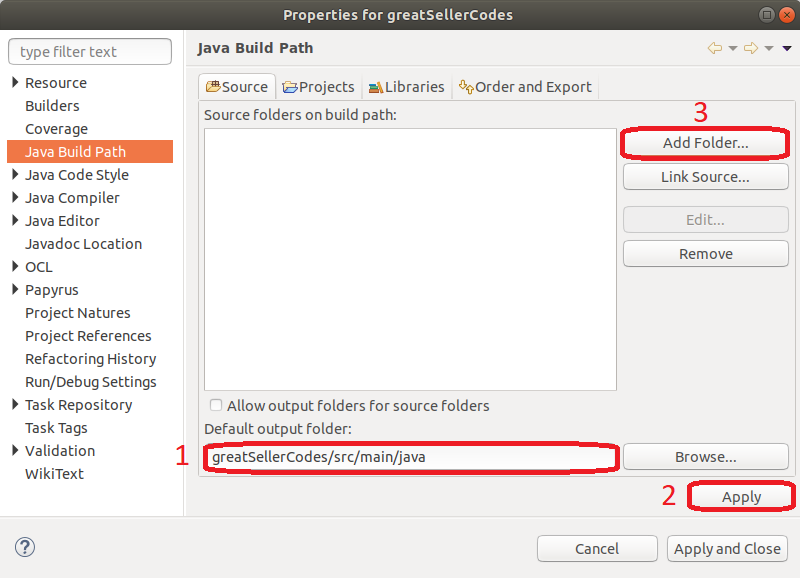
\includegraphics[scale=0.3]{./chapter4/projPapyrus/Selection_004.png}}
\caption{Representation Kind}
\label{fig:Representation Kind}
\end{figure}

Finally, we can finish with the new Papyrus project initialization (figure \ref{fig:Papyrus Project Definition}).

\begin{figure}
\centering
{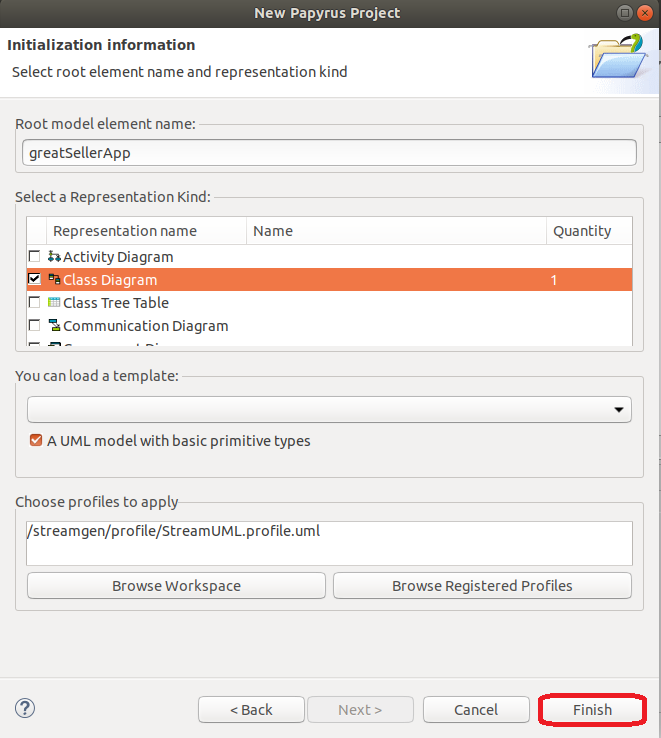
\includegraphics[scale=0.3]{./chapter4/projPapyrus/Selection_005.png}}
\caption{Papyrus Project Definition}
\label{fig:Papyrus Project Definition}
\end{figure}

The next step is to define the model in the class diagram in order to specify that the application is going to be a Flink application. Then, first of all, we have to create a model node in the greatSellerApp.di file. This node is going to be called greatSeller as it is the object representing the whole application. Once the node is inserted, the properties of such node must be specified. More in detail, the Flink application stereotype has to be applied. In this case, the properties of the model has to be the default ones then nothing else must be done with the model node.

The next step is to add the data types that the application is going to need. In order to do this, a package node has to be inserted inside the Flink application model node. This package is called greatSellerDataTypes and a stereotype has to be applied as in the previous case. First of all, inside the properties windown, in the profile field, the applied stereotype is defined. Inside this package all the datatypes that the application requires have to be inserted. The first data type is the InputTransactions which is composed of a transaction id (integer), a data subject (string), an amount (double) and a recipient id (string). The second data type is the IssuedTransactions which contains the data subject (string) and the number of transactions performed by such data subject which can be seen by means of the variable NTransactions (integer). The third data type is the SpentAmount which is composed of the data subject (string) and the total amount of money spent by the data subject which can be seen by means of the variable TotalAmount (double). Finally, the last data type is the NumberUsers which contains the number of users who spent more than 1000 dollars and it is represented by means of the variable NTopUsers (integer). Then, we need to insert one DataType node inside the package created in the previous step with each of these data types. Each data type can be seen as a tuple which is composed by several values. The name of the DataType node is going to be the same that the one corresponding to the tuple and each of the values that compose the tuple are going to be a property inside of the owned attributes that are specified in the UML field of the properties of each DataType node.

\begin{table}[h!]
\centering
	\begin{tabular}{||c|c|c||} 
	\hline\hline
	DataType & Properties & PropertyType \\ [1ex] 
	\hline\hline
	InputTransactions & transactionId & integer  \\
	& dataSubject & string  \\
	& amount & double  \\
	& recipientId & string  \\
	\hline
	IssuedTransactions & dataSubject & string  \\
	& nTransactions & integer \\
	\hline
	SpentAmount & dataSubject & string  \\
	& totalAmount & double \\
	\hline
	NumberUsers & NTopUsers & double  \\
	\hline\hline
	\end{tabular}
\caption{DataTypes Composition}
\label{DataTypes Composition}
\end{table}


\chapter{Evaluation}

\section{Great Seller DIA}

In this section a DIA for an e-commerce company called Great Seller is implemented. This DIA is able to compute real time statistics about the transactions generated by the consumers. Such statistics can be observed by some other companies that pay in order to have access to the information making that Great Seller acts as a data broker. In order to simplify the implementation, Great Seller is going to sell three different types of statistics:

\begin{itemize}

\item Statistic 1: the total amount of money that each consumer of Great Seller spend in the last 10 minutes.
\item Statistic 2: the number of transactions issued by each user in the last 10 minutes.
\item Statistic 3: the number of users who spent more than \euro{1000} in the last hour.

\end{itemize}

As any DIA, Great Seller generates such statistics by some transformations which are fed from a source and the generated information is stored into a sink which is accessible by the observer companies. Moreover, as Great Seller is producing three different types of statistics, its DIA requires three different sinks where the information should be stored. Due to the fact that Great Seller DIA is computing real time statistics about the transactions that are generated by the consumers of the company, only one source is required for the DIA model. Finally, one transformation is necessary for the computation of each statistic. In summary, Great Seller DIA requires one source, three transformations and three sinks for the design of its model.

\subsection{Great Seller Source}
In the implementation described along this document, Great Seller DIA is fed from a socket that reads from a text file where all the transactions generated by the consumers of Great Seller are stored. All the transactions are going to have the same predefined tuple structure 'transactionId,dataSubject,spentAmount,purchasedProduct'. This predefined structure is represented in the Great Seller DIA model by means of a Data Type called InputTransaction.

Regarding to the fields of such tuple, the transactionId field is an integer which varies from 1 to the number of generated transactions, such number can be 10, 100 or 1000. The dataSubject is the user who generates such tuple and it is one of the following: Bob, Carlos, Elisabetta or Michele. The spentAmount is the price paid for the product bought with the transaction and it is an integer with a low boundary of \euro{1} and an upper boundary of \euro{200}. Finally, the purchasedProduct is the product bought with such transaction.

It is important to remark that socket source introduces in the DIA a data stream of string and the InputTransaction Data Type must be generated by means of a transformation which parses the string into the Data Type. This transformation is called TupleParser as it splits the incoming tuples, strings, into the InputTransaction Data Type.

The Great Seller stock is composed by means of 25 products. In order to simplify the implementation, each product is named by the word 'product' immediately followed by a number between 1 and 25 in order to specify the product referred in the stock. In the table \ref{Great Seller Stock} can be seen such stock.

\begin{table}[h!]
\centering
	\begin{tabular}{||c|c||} 
	\hline\hline
	Product & Price (\euro{}) \\ [1ex] 
	\hline\hline
	product1 & 196 \\ 
	\hline
	product2 & 36 \\ 
	\hline
	product3 & 179 \\ 
	\hline
	product4 & 17 \\ 
	\hline
	product5 & 120 \\ 
	\hline
	product6 & 187 \\ 
	\hline
	product7 & 139 \\ 
	\hline
	product8 & 52 \\ 
	\hline
	product9 & 160 \\ 
	\hline
	product10 & 110 \\ 
	\hline
	product11 & 113 \\ 
	\hline
	product12 & 67 \\ 
	\hline
	product13 & 100 \\ 
	\hline
	product14 & 125 \\ 
	\hline
	product15 & 192 \\ 
	\hline
	product16 & 115 \\ 
	\hline
	product17 & 113 \\ 
	\hline
	product18 & 98 \\ 
	\hline
	product19 & 113 \\ 
	\hline
	product20 & 185 \\ 
	\hline
	product21 & 143 \\ 
	\hline
	product22 & 18 \\ 
	\hline
	product23 & 194 \\ 
	\hline
	product24 & 41 \\ 
	\hline
	product25 & 26 \\ 
	\hline\hline
	\end{tabular}
\caption{Great Seller Stock}
\label{Great Seller Stock}
\end{table}

\subsection{Great Seller Transformations}
In order to compute each of the three statistics that Great Seller sells as data broker, the Great Seller DIA needs three transformations. Each of this transformations is the operator of each statistic. Thus, the operator one (OP1) computes the total amount of money spent by each user in the last 10 minutes. The second operator (OP2) computes the number of transactions issued by each user in the last 10 minutes. Finally, the operator three (OP3) computes the number of users who spent more than \euro{1000} in the last hour.

These transformations input a data stream with a set of tuples that all of them have identical structure. Thus, the first stream (S1) is composed of tuples of the kind InputTransaction. This stream is duplicated and it is sent to the operators OP1 and OP2. Moreover, as each operator works taking into account the data subject of each tuple, the stream S1 must be keyed by the data subject field of this first stream. Finally, as the operators have to compute the statistics taking into account only the tuples generated in the last 10 minutes, the stream S1 is windowed by a time window of 10 minutes.

The new data generated in the OP1 are represented in a new data type called SpentAmount and that is composed by two fields following the structure: 'dataSubject, totalAmount'. The SpentAmount tuples are collected in the stream S2 and they are keyed by the data subject field of such stream.

Finally, the data generated in the OP2, is collected in a new data type called IssuedTransaction whose structure is 'dataSubject, nTransactions'. This new stream (stream S3) is sent to the OP3. Moreover, this third stream is keyed by the data subject field of the stream and it is also windowed with a time window of one hour. The OP3 generates a randomly partitioned stream with an uniform distribution called stream S4 whose structure is: 'nTopUsers'.

\subsection{Great Seller Sinks}
Each of the tuples flowing through the DIA must be stored in a file, in order to be able to access to the tuples that will be sent to the observer companies. This is why, after each generated stream, a file text sink is implemented with different paths in order to store each of the flows obtaining all the results in three different files. The file with the results of the stream S2, the stream S3 and the stream S4.
This implementation is given due to the fact that each of the tuples generated by the operators are observable for the observer companies who buy them.

In the figure \ref{fig:Great Seller Dataflow model} the dataflow model of the Great Seller DIA without privacy policies can be seen. This dataflow model can be found in \cite{privacypoliciesarticle}. On the other hand, in the figure \ref{fig:Great Seller StreamGen DIA} the model developed with StreamGen taking into account the figure \ref{fig:Great Seller Dataflow model} can be seen for such DIA.

\begin{figure}
\centering
{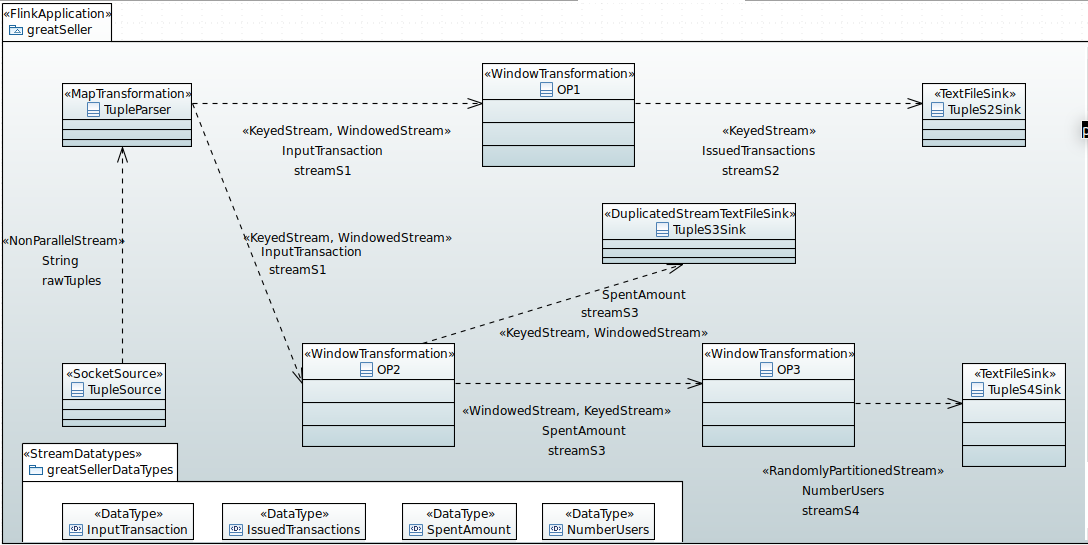
\includegraphics[scale=0.3]{./chapter3/greatSellerStreamGen.png}}
\caption{Great Seller StreamGen DIA}
\label{fig:Great Seller StreamGen DIA}
\end{figure}

\subsubsection*{Great Seller DIA Limitations}

After developing this DIA, some limitations are identified relative to the current development of StreamGen. The first limitation is the number of servers that can be connected directly to a Map Transformation. In this example, it is supposed that the users send the transactions by means of a server to the target DIA. This server is the same for all the users who are using Great Seller DIA. At this point, a casuistry is proposed. This is the case of a DIA involved in an industry 4.0 application where the owner of the factory cannot afford to invest in a server for the DIA and all the machines generating datasets must be connected directly to the DIA by means of the factory net.

The second limitation that is extracted is that StreamGen does not allow to generate float or double data types. In this example, Great Seller is working with a stock where all the products have integer prices but should be necessary a DIA which allows, among the language, to declare float or double values.

The last extracted limitation is that StreamGen is not able to handle the privacy of the users who are using the DIA. In this case, neither the language for such purpose nor the translation by means of Acceleo are available. After the development of both things, this model should be reused in order to make the application privacy aware.

\section{Cool Analyst DIA}

In addition to Great Seller, another DIA is developed with StreamGen. This is the case of Cool Analyst, a DIA which is able to compute some statistics from the temperatures measured in two different refrigeration chambers of a panettone factory called Panettone 4.0. These measurements are going to be stored in a CSV file in order to be accessible by the manager of the industrial plant to see if any problem has been produced in the yeast fermentation. This application is going to compute four statistics in two different operators:

\begin{itemize}
\item Operator 1: the maximum, the minimum and the average temperature of each chamber during the last 5 minutes.
\item Operator 2: the prediction of the temperature for the next 10 minutes.
\item Operator 3: the filtered data between a range which have no null value and no null id.
\end{itemize}

Cool Analyst DIA is going to require two socket sources, one for each of the industrial chambers, two transformations in order to compute each of the operators specified before and two sinks where the CSV files with each of the results of the operators can be stored. For the development of the prediction operator, as its development is out of this document, it is taken from an already working transformation for such purpose.

\subsection{Cool Analyst Sources}

Panettone 4.0 is using temperature digital sensors in each of its two chambers where yeasts are fermented. These sensors are connected to the net of the factory and are sending the measured values directly to the Cool Analyst DIA with a 1 second sample frequency.

This two chambers need to control the temperature of the room in order to allow the correct fermentation of the yeasts. The role of the first chamber is to make the primary fermentation in the production process of the Panettone 4.0 factory. This fermentation is also known as bulk fermentation. On the other hand, the role of the second camera is to make the secondary fermentation which is also known as proofing. More information can be read about the fermentation of the years and how to control the temperature during its production in \cite{yeastfermentation}. The conclusions that are extracted from \cite{yeastfermentation}, and that are useful for our purpose, are that the bulk fermentation must have the temperatures of the room in the range [20, 24] Celsius whilst the secondary fermentation must have an environment with temperatures in the range [22, 29] Celsius. This is why Cool Analyst requires two socket sources connected to the port and to the host of each of the chambers.

Also it is important to remark how the temperatures of the chambers are simulated. For such purpose a python code has been developed. This model takes as target temperature, the average temperature of each of the ranges. This temperature is supposed to be maintained during thirty seconds. Then, randomly, the program generates a sine function with a frequency of 1/16 Hz for the lower range and with a frequency of 1/28 Hz for the upper range. The lower range is considerate from the lower boundary of each of the ranges of temperature that the chambers can admit until the average temperature and the upper range from the average temperature until the upper boundary of the ranges. In the figures \ref{fig:Temperature Chamber 1 Model} and \ref{fig:Temperature Chamber 2 Model} can be seen both models.

\begin{figure}
\centering
{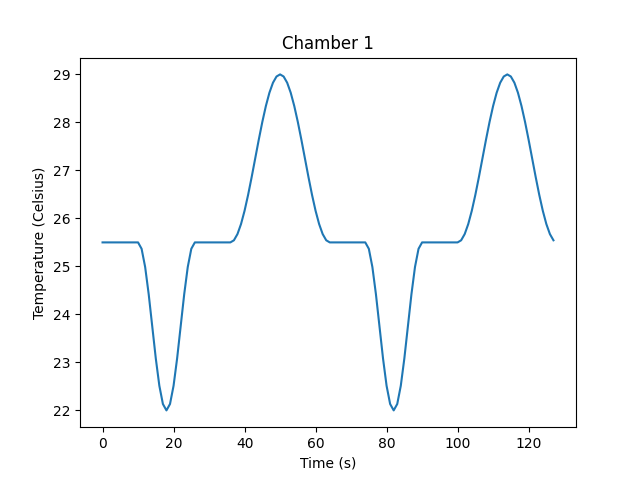
\includegraphics[scale=0.3]{./chapter3/room1TempModel.png}}
\caption{Temperature Chamber 1 Model}
\label{fig:Temperature Chamber 1 Model}
\end{figure}

\begin{figure}
\centering
{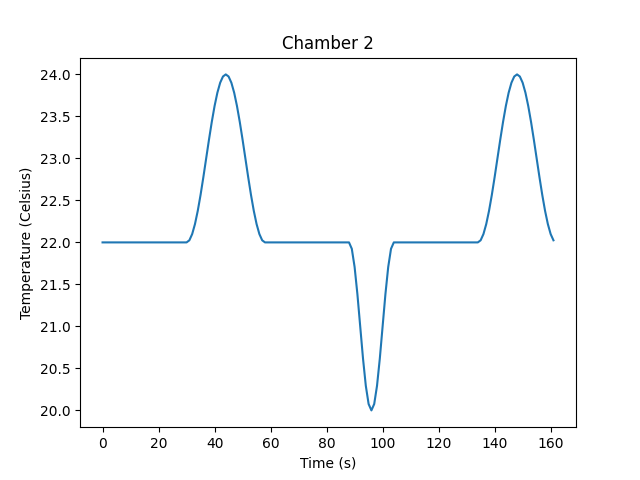
\includegraphics[scale=0.3]{./chapter3/room2TempModel.png}}
\caption{Temperature Chamber 2 Model}
\label{fig:Temperature Chamber 2 Model}
\end{figure}

Finally, these two models have been generated and saved in a TXT file which is going to be read from the Python servers that have been developed in order to simulate the chambers. These servers are going to read one value each second. This will generate that the socket sending the values from the chamber 1 stops earlier than the other socket. This model design will allow to proof the right behavior of the whole application. Allowing to see what would happen if, suddenly, the sensors are disconnected.

\subsection{Cool Analyst Transformations}

The values read from the TXT file are sent in a string which has to be parsed in order to generate the Data Types that are used in the DIA. The strings contain the roomId followed by the temperature and both values are separated by means of a comma. This is why, first of all a NMap Transformation has been developed, this will be explained in the following chapter. This NMap transformation inputs the two streams with the strings sent by the room servers and the string is parsed into a roomTemp data type which is composed of two properties: roomId (string) and roomTemp(double). In order to introduce double values from the Papyrus model by means of StreamGen, in chapter 4 is explained how StreamGen was modified.

Once the roomTemp data type is generated, a stream is sent to a window transformation called RoomStatistics. In this transformation all the computations explain in the operator 1 are calculated (maximum temperature, minimum temperature and average temperature). This transformation generates a new data type called roomStatistics which is composed of four properties: roomId (string), maxTemp (double), minTemp (double) and avgTemp (double).

Then, the stream with the roomStatistics data types is sent to the TemperaturePredictor transformation. This window transformation computes the operations described in the operator 2 and generates the tempPred data type. This data type is composed of two properties: roomId (string) and predTemp (double).

The last operator takes the stream with the roomTemp data type and, by means of a filter transformation called CleanRawData, checks that there is no temperature with a value below -9999 neither 9999. Moreover, this transformation checks that the temperature has a value and that value is referenced to a room identifier.

\subsection{Cool Analyst Sinks}

Finally, the data types generates in the RoomStatistics, in the TemperaturePredictor and in the CleanRawData transformations are stored each one in its sink. Cool Analyst uses CSV sinks as this kind of files are commonly used by engineers who work in the factories. In order to do this, the output stream from the RoomStatistics transformation is sent to StatisticsSink where is specified the path of the generated file, the output stream from the TemperaturePredictor transformation is sent to PredictorSink where the path of the second output file is specified and the same proceadure is done with the third operator CleanRawData and its sink CleanDataSink.

In the figures \ref{fig:Cool Analyst Dataflow model} and \ref{fig:Cool Analyst StreamGen DIA} can be seen the Cool Analyst Dataflow Model and the Cool Analyst StreamGen DIA explained above.

\begin{figure}
\centering
{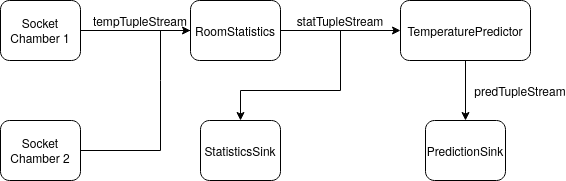
\includegraphics[scale=0.5]{./chapter3/coolAnalystApp.png}}
\caption{Cool Analyst Dataflow model}
\label{fig:Cool Analyst Dataflow model}
\end{figure}

\begin{figure}
\centering
{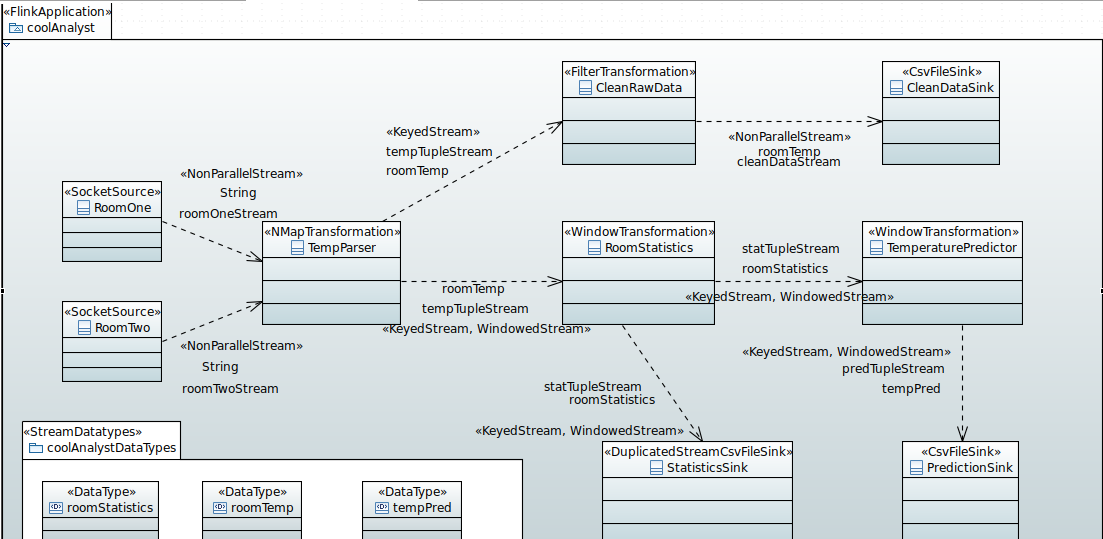
\includegraphics[scale=0.3]{./chapter3/coolAnalystStreamGen.png}}
\caption{Cool Analyst StreamGen DIA}
\label{fig:Cool Analyst StreamGen DIA}
\end{figure}

\subsubsection*{Great Seller DIA Limitations}

At this example two of the limitations identified with the previous DIA are already solved. This is the case of the NMap Transformation and the possibility to generate double values by means of Papyrus. This will be seen in the following chapter.

However, StreamGen is still not able to handle the privacy of the users who are using the DIA. This is why this DIA will be reused, as Great Seller, after the development of the language and the Acceleo code to test StreamGen for privacy purposes.



\chapter{Conclusion}
\chapter[Chapter 6]{Conclusions}
\label{sec:conclusions}


\begin{thebibliography}{9}

\bibitem{hadoopwebsite} 
Hadoop Tutorial
\\\texttt{https://data-flair.training/blogs/hadoop-tutorial/}

\bibitem{sparkwebsite} 
Spark Tutorial
\\\texttt{https://data-flair.training/blogs/spark-tutorial/}

\bibitem{flinkwebsite} 
Apache Flink Tutorial
\\\texttt{https://data-flair.training/blogs/apache-flink-tutorial/}

\bibitem{privacypoliciesarticle} 
Michele Guerriero, Damian Andrew Tamburri, Elisabetta Di Nitto.
\textit{Defining, Enforcing and Checking Privacy Policies In Data-Intensive Applications}. 
13th International Symposium on Software Engineering for Adaptive and Self-Managing Systems, 2018.

\bibitem{modelwebsite} 
Modeling Tutorial
\\\texttt{https://www.transentis.com/methods-techniques/models-and-metamodels/}

\bibitem{umlwebsite} 
Unified Modeling Language Tutorial
\\\texttt{https://www.visual-paradigm.com/guide/uml-unified-modeling-language/what-is-uml/}

\bibitem{metamodelwebsite} 
Metamodeling Platforms
% http://www.dke.univie.ac.at/mmp/FullVersion_MMP_DexaECWeb2002.pdf
\\\texttt{http://www.dke.univie.ac.at/mmp/FullVersion\char`_MMP\char`_DexaECWeb2002.pdf}

\end{thebibliography}


\end{document}
